\documentclass[a4paper,9pt]{extarticle}

%=========================================================
% PACKAGES
%=========================================================

\usepackage[
a4paper,
top=1.8cm,
bottom=1.5cm,
footskip=7mm,
left=1cm,
right=1cm,
headheight=14pt,
headsep=5mm
]{geometry}
\usepackage[T1]{fontenc}
\usepackage[utf8]{inputenc}
\usepackage[french]{babel}

\usepackage[sfdefault]{FiraSans}
\renewcommand{\familydefault}{\sfdefault}

\usepackage{multicol}
\setlength{\columnsep}{0.7cm}

\usepackage{amsmath,amssymb}

\usepackage{titlesec}
\usepackage{enumitem}

\usepackage{tcolorbox}
\tcbuselibrary{skins,breakable}

\usepackage{xcolor}

\usepackage{graphicx}
\usepackage{float}

\usepackage{tikz}

\usepackage{fancyhdr}
\usepackage[hidelinks]{hyperref}


%=========================================================
% PAGE SETTINGS
%=========================================================

\setlength{\parindent}{0pt}
\setlength{\parskip}{1.5pt}

\setlength{\abovedisplayskip}{4pt}
\setlength{\belowdisplayskip}{4pt}

\setlist[itemize]{
leftmargin=*,
itemsep=1pt,
topsep=1pt
}


%=========================================================
% COLORS
%=========================================================

\definecolor{Blue}{HTML}{E3F0FF}
\definecolor{Green}{HTML}{E3F7EA}
\definecolor{Pink}{HTML}{FFE5ED}
\definecolor{Orange}{HTML}{FFF0DC}
\definecolor{Purple}{HTML}{EEE7FF}
\definecolor{Yellow}{HTML}{FFFADB}


\definecolor{BlueTitle}{HTML}{285B8F}
\definecolor{GreenTitle}{HTML}{287052}
\definecolor{PinkTitle}{HTML}{A84063}
\definecolor{OrangeTitle}{HTML}{A96500}
\definecolor{PurpleTitle}{HTML}{6245A5}


%=========================================================
% HEADER
%=========================================================

\pagestyle{fancy}

\fancyhf{}

\fancyhead[L]{\small\textbf{Numerical Methods}}
\fancyhead[C]{\small Linear Systems III}
\fancyhead[R]{\small Week 04 --- 28/09-04/10/2026}

\fancyfoot[C]{\small\href{https://github.com/AlphaXT38G/notes_ba5}{github.com/AlphaXT38G/notes\_ba5}}
\fancyfoot[R]{\small \thepage}

\renewcommand{\headrulewidth}{0.4pt}



%=========================================================
% TITLES
%=========================================================

\titleformat{\section}
{\large\bfseries\color{BlueTitle}}
{}{0pt}{}

\titlespacing{\section}
{0pt}{6pt}{3pt}


% separator

\newcommand{\separator}{
\vspace{2pt}
\hrule
\vspace{3pt}
}


%=========================================================
% BOXES
%=========================================================

% Boxes are kept whole (unbreakable): inside multicols, a box split by tcolorbox
% leaves an empty column behind it.

% DEFINITION - blue
\newtcolorbox{definition}{
enhanced,
unbreakable,
colback=Blue,
colframe=BlueTitle,
boxrule=0.7pt,
arc=0mm,
title=\textbf{Definition},
fonttitle=\bfseries
}

% IMPORTANT - pink
\newtcolorbox{important}{
enhanced,
unbreakable,
colback=Pink,
colframe=PinkTitle,
boxrule=0.7pt,
arc=0mm,
title=\textbf{Key idea},
fonttitle=\bfseries
}

% FORMULAS - green
\newtcolorbox{formula}{
enhanced,
unbreakable,
colback=Green,
colframe=GreenTitle,
boxrule=0.7pt,
arc=0mm,
title=\textbf{Key formulas},
fonttitle=\bfseries
}

% WARNING - orange
\newtcolorbox{warning}{
enhanced,
unbreakable,
colback=Orange,
colframe=OrangeTitle,
boxrule=0.7pt,
arc=0mm,
title=\textbf{Warning},
fonttitle=\bfseries
}

% EXAMPLE - purple
\newtcolorbox{example}{
enhanced,
unbreakable,
colback=Purple,
colframe=PurpleTitle,
boxrule=0.7pt,
arc=0mm,
title=\textbf{Example},
fonttitle=\bfseries
}

% SUMMARY - orange
\newtcolorbox{summary}{
enhanced,
unbreakable,
colback=Yellow,
colframe=OrangeTitle,
boxrule=0.7pt,
arc=0mm,
title=\textbf{Summary},
fonttitle=\bfseries
}



%=========================================================
% FIGURE BOX
%=========================================================

\newtcolorbox{figurebox}{
enhanced,
colback=white,
colframe=gray,
boxrule=0.5pt,
arc=0mm,
center
}



%=========================================================
% DOCUMENT
%=========================================================

\begin{document}

%\footnotesize   --> To reduce the size of the text

\thispagestyle{fancy}



% Columns keep their natural height: boxes are unbreakable, stretching would open gaps.
\raggedcolumns
\begin{multicols}{2}


%=========================================================
\section{Recap: Normal Equations}


Homework 2 out today (processing a RAW image). Lecture topics: least squares problems,
orthogonality, polynomial regression. \textbf{Common theme today: orthogonality.}


\begin{formula}

The ``best'' solution (in the $L_2$ sense) of a tall system is given by

\[
\mathbf{A}^T\mathbf{A}\mathbf{x} = \mathbf{A}^T\mathbf{b}
\]

\end{formula}


\begin{important}

The normal equations yield a symmetric \emph{quadratic} linear system, whose size is given by
the number of columns of $\mathbf{A}$. Geometrically, $\mathbf{y} = \mathbf{A}\mathbf{x}$ is the
point of $\operatorname{span}(\mathbf{A})$ closest to $\mathbf{b}$: the residual
$\mathbf{r}(\mathbf{x})$ is perpendicular to it.

\end{important}


\textbf{Regression and its limitations}: overfitting, wrong model.

\begin{center}

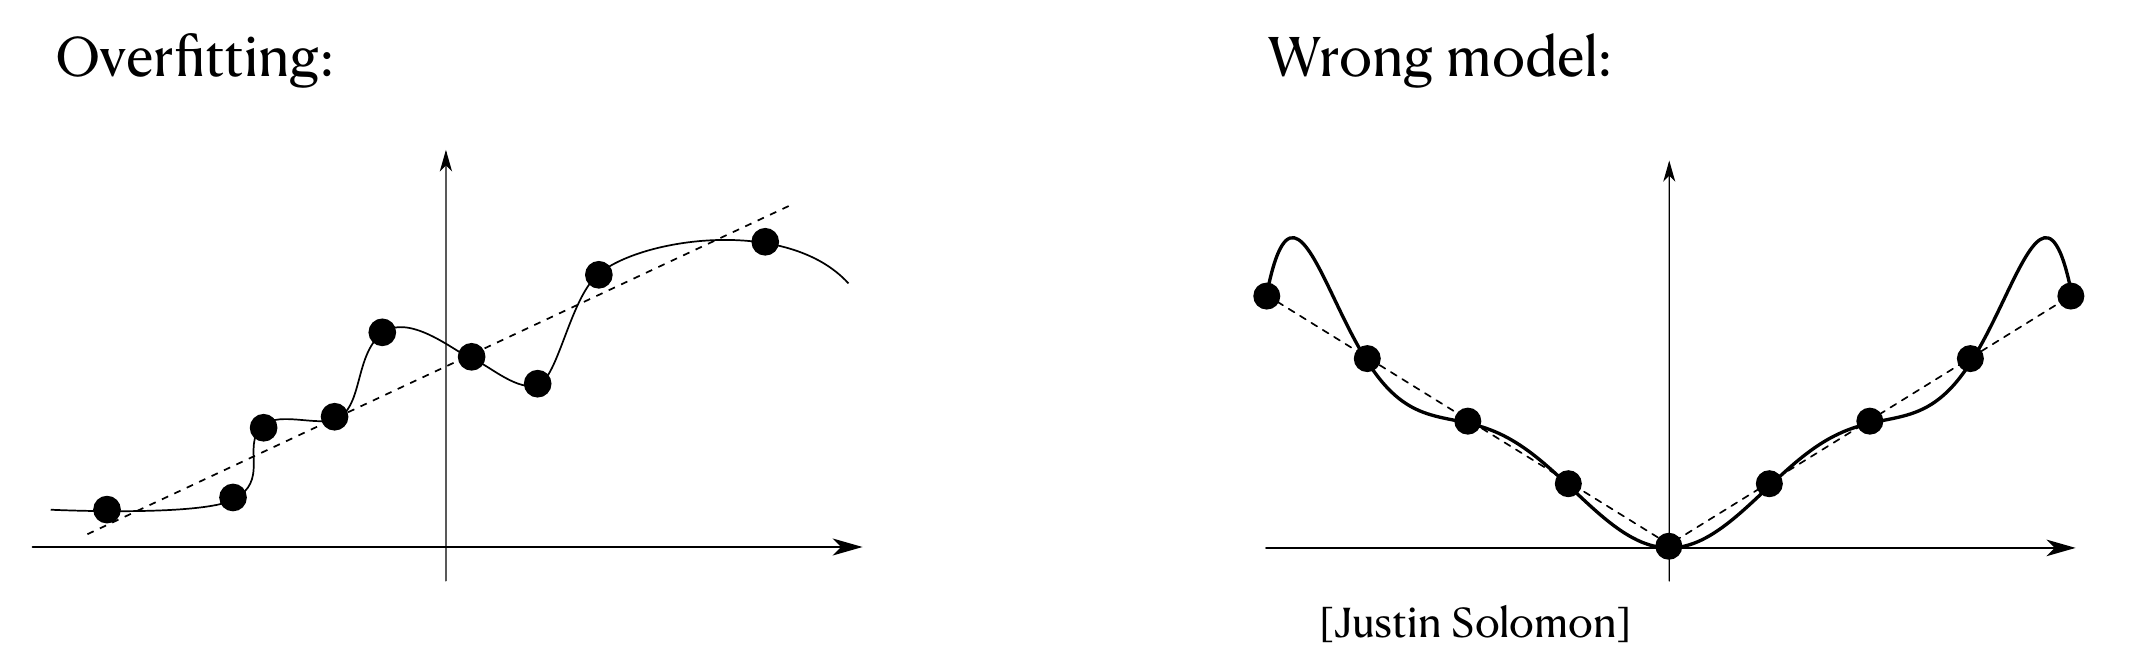
\includegraphics[
width=0.9\linewidth
]{../images/week04_01.png}

\end{center}


\begin{warning}

\textbf{Okay, so what's the catch?}

\[
\operatorname{cond}(\mathbf{A}^T\mathbf{A}) \approx \operatorname{cond}(\mathbf{A})^2
\]

The condition number of a problem expressed using the normal equations is often \emph{much
worse} than the condition number of the original problem.

\end{warning}


\begin{important}

\textbf{One of our goals for today}: can we solve the same problem, but without ever building
$\mathbf{A}^T\mathbf{A}$?

\end{important}



%=========================================================
\section{Orthogonality}


\textbf{The issue with the Vandermonde matrix} (geometric interpretation): monomials of
different powers look more and more alike, so the columns are almost parallel. \textbf{Idea}:
somehow make the problem more ``orthogonal''.

\begin{center}

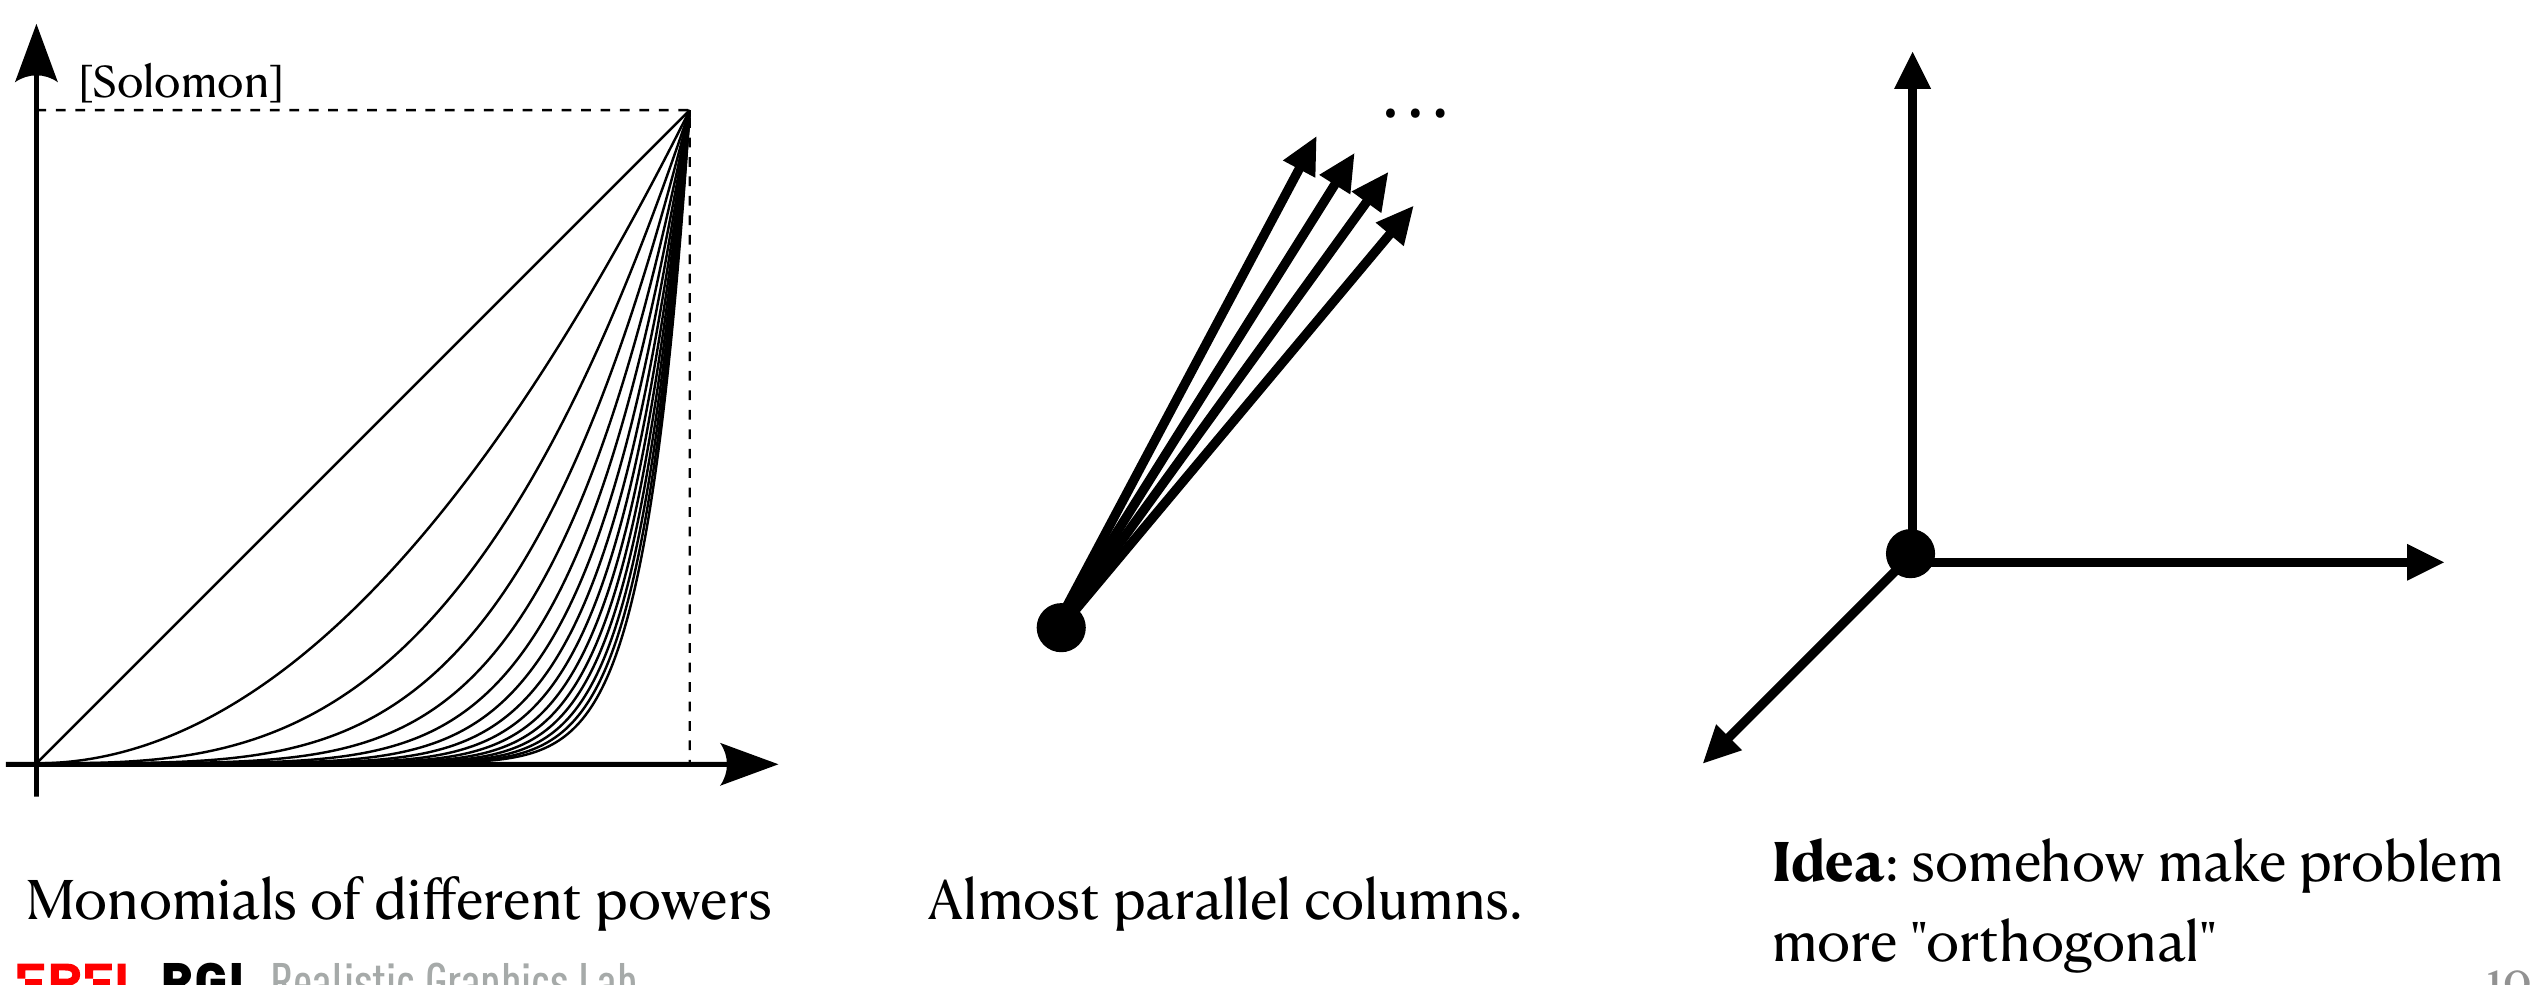
\includegraphics[
width=\linewidth
]{../images/week04_02.png}

\end{center}


\begin{definition}

\textbf{INNER PRODUCT} (measures a projection)

\[
\langle \mathbf{a}, \mathbf{b} \rangle = \mathbf{a} \cdot \mathbf{b} = \mathbf{a}^T\mathbf{b}
= \|\mathbf{a}\|\,\|\mathbf{b}\| \cos\theta
\]

\begin{itemize}

\item If $\mathbf{a}$ has unit length, $\mathbf{a}^T\mathbf{a} = 1$.

\item If $\mathbf{a}$ and $\mathbf{b}$ are perpendicular, $\mathbf{a}^T\mathbf{b} = 0$.

\end{itemize}

\end{definition}



%=========================================================
\section{Gram-Schmidt Orthogonalization}


\begin{definition}

\textbf{GRAM-SCHMIDT STEP}

\[
\hat{\mathbf{y}} := \mathbf{y} - \frac{\langle \mathbf{x}, \mathbf{y} \rangle}
{\langle \mathbf{x}, \mathbf{x} \rangle}\mathbf{x}
\]

Then $\langle \mathbf{x}, \hat{\mathbf{y}} \rangle = 0$: remove from $\mathbf{y}$ its projection
on $\mathbf{x}$.

\end{definition}


\begin{example}

$\mathbf{x} = (1, 2, 3)^T$, $\mathbf{y} = (4, 5, 6)^T$:
$\langle \mathbf{x}, \mathbf{y} \rangle = 1 \cdot 4 + 2 \cdot 5 + 3 \cdot 6 = 32$.

\end{example}


\begin{definition}

\textbf{INNER PRODUCTS ARE MORE GENERAL}

\[
\langle \mathbf{x}, \mathbf{y} \rangle := \sum_{i=1}^{n} x_i y_i
\qquad
\langle f, g \rangle := \int_a^b f(x) g(x)\,\mathrm{d}x
\]

\end{definition}



%=========================================================
\section{Gram-Schmidt Applied to Polynomials}


\begin{formula}

Everything defined on $[-1, 1]$. Input (monomials): $f(x) = 1$, $g(x) = x$, $h(x) = x^2$.

\begin{align*}
\langle f, g \rangle &= \int_{-1}^{1} 1 \cdot x\,\mathrm{d}x
= \left[\tfrac{1}{2}x^2\right]_{-1}^{1} = 0 \\
\langle g, h \rangle &= \int_{-1}^{1} x \cdot x^2\,\mathrm{d}x
= \left[\tfrac{1}{4}x^4\right]_{-1}^{1} = 0 \\
\langle f, h \rangle &= \int_{-1}^{1} 1 \cdot x^2\,\mathrm{d}x
= \left[\tfrac{1}{3}x^3\right]_{-1}^{1} = \tfrac{2}{3}
\end{align*}

\[
\hat{h}(x) = h(x) - \frac{\langle f, h \rangle}{\langle f, f \rangle}f(x) = x^2 - \frac{1}{3}
\]

\end{formula}


\begin{definition}

\textbf{LEGENDRE POLYNOMIALS}

\begin{itemize}

\item Span the same domain as monomials, but they are \textbf{orthogonal to each other}!

\item Problems with poor condition number disappear completely!

\item Use them when you need to fit a smooth function to some data.

\end{itemize}

\end{definition}


\begin{center}

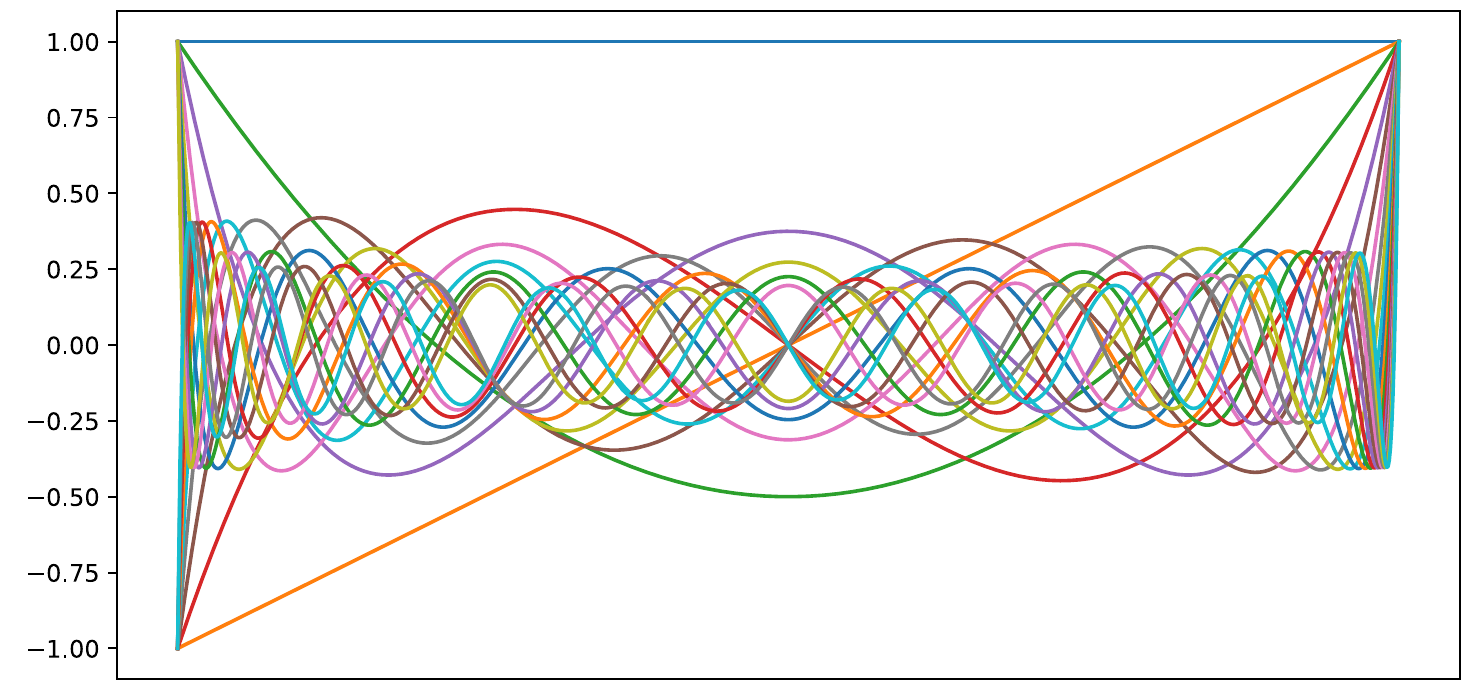
\includegraphics[
width=0.8\linewidth
]{../images/week04_03.png}

\end{center}



%=========================================================
\section{Runge Function and Chebyshev Points}


Demo: the Runge function, fitted by polynomials through uniformly spaced points.


\begin{definition}

\textbf{TAYLOR'S THEOREM}

Approximation of a function around a point $a$. The residual of the approximation is equal to the
$k{+}1^{\text{st}}$ derivative \emph{somewhere} between the expansion point and where the function
is evaluated. What about the error away from this point?

\end{definition}


\begin{formula}

\textbf{Taylor's theorem for polynomials} (approximation around a sequence of points
$x_i$ used for the fit):

\[
R_{k-1}(x) = \frac{f^k(y)}{k!}\prod_{i=1}^{k}|x - x_i|
\]

\textbf{Idea}: try to make $\prod_{i=1}^{k}|x - x_i|$ small. \textbf{Optimal} set of points
that achieve this (\textbf{Chebyshev points}):

\[
x_i = \cos\left(\frac{2k - 1}{2n}\pi\right)
\]

\end{formula}


\begin{important}

Demo, Runge function part II: using Chebyshev points instead of uniformly spaced ones.

\end{important}



%=========================================================
\section{The QR Decomposition}


\begin{definition}

\textbf{QR FACTORIZATION}

\[
\mathbf{A} = \mathbf{Q}\mathbf{R}
\]

\begin{itemize}

\item \emph{Different flavors exist}: Gram-Schmidt, Givens rotations, \textbf{Householder
transformations}.

\item Follows the previous approach of using (pre-)computation to transform a ``difficult''
linear system into one that has a special structure, making it ``easy''.

\item Compared to LU, one triangular factor was replaced by an \textbf{orthogonal matrix}.

\end{itemize}

\end{definition}


\begin{formula}

\[
\mathbf{Q} = \begin{pmatrix} | & & | \\ \mathbf{q}_1 & \cdots & \mathbf{q}_n \\ | & & |
\end{pmatrix}
\]
\[
\mathbf{Q}^T\mathbf{Q} = \begin{pmatrix}
\mathbf{q}_1^T\mathbf{q}_1 & \cdots & \mathbf{q}_1^T\mathbf{q}_n \\
\vdots & & \vdots \\
\mathbf{q}_n^T\mathbf{q}_1 & \cdots & \mathbf{q}_n^T\mathbf{q}_n
\end{pmatrix} = \mathbf{I}
\]

\end{formula}


\begin{important}

Orthogonal transformations preserve distances, angles. They do \textbf{not} amplify error!

\end{important}


\begin{definition}

\textbf{ISOMETRY}

A transformation that preserves angles \& distances. Rotate, mirror: isometric. Shear (and
scaling): \textbf{not} isometric.

\end{definition}


\begin{warning}

\textbf{The problem}: least squares problems seek the solution in
$\operatorname{span}(\mathbf{A})$ that is \emph{closest} to $\mathbf{b}$. If we
non-isometrically transform the problem (as the LU decomposition does), then that actually
changes the answer\dots

\end{warning}



%=========================================================
\section{Householder Reflections}


\begin{important}

\textbf{The challenge}: like LU, make $\mathbf{A}$ upper triangular (``R'' as in \emph{right
triangular}, the same as upper-triangular), column by column:

\[
\mathbf{Q}\mathbf{x} = \mathbf{Q}\begin{pmatrix} x_1 \\ x_2 \\ \vdots \\ x_n \end{pmatrix}
= \begin{pmatrix} \tilde{x}_1 \\ 0 \\ \vdots \\ 0 \end{pmatrix}
\]

\textbf{Goal}: zero out all elements of $\mathbf{x}$ except for the first. \textbf{Challenge}: need
to do this only using rotations or reflections.

\end{important}


\begin{center}

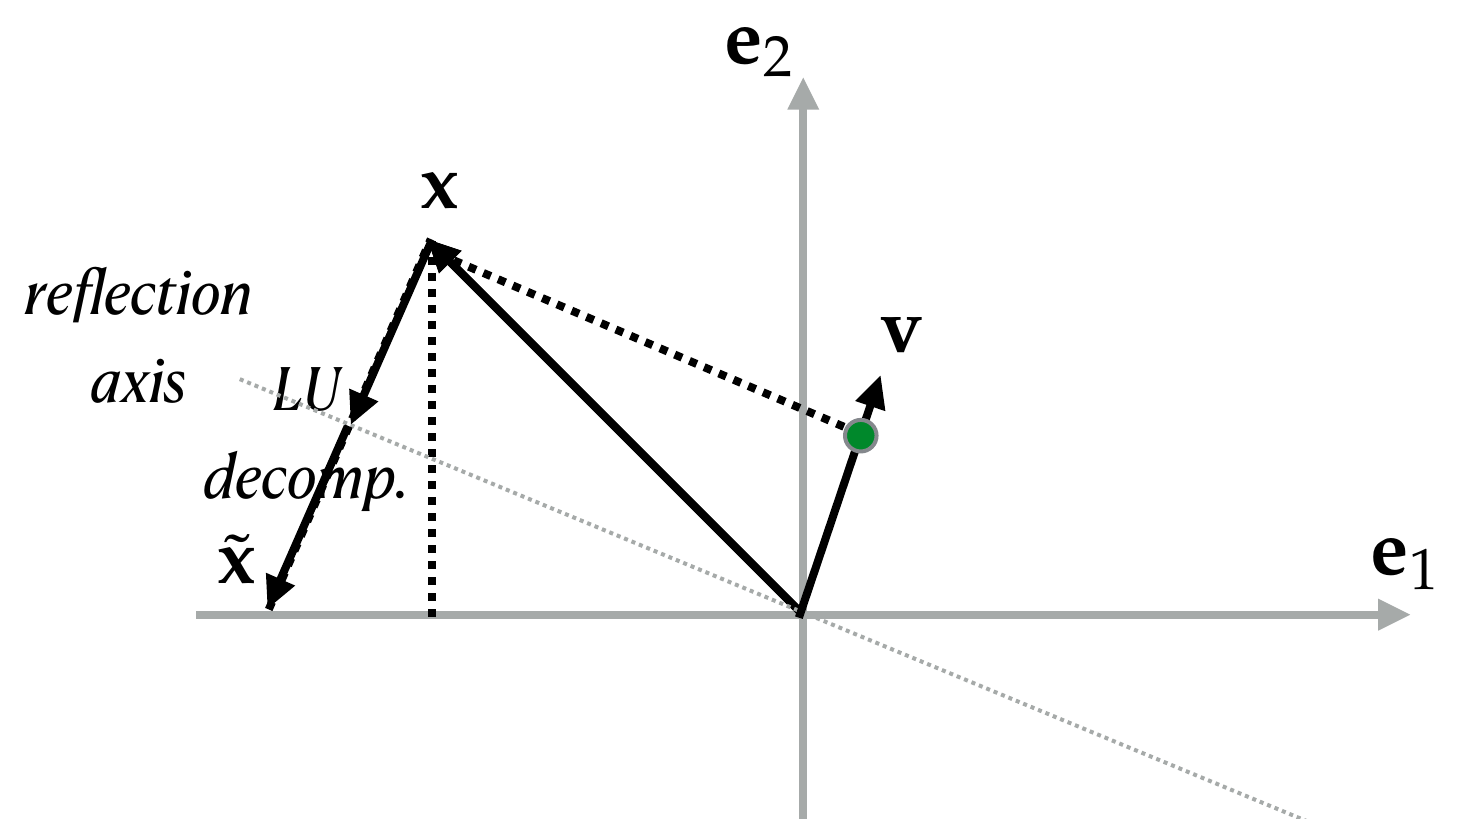
\includegraphics[
width=0.7\linewidth
]{../images/week04_04.png}

\end{center}


\begin{definition}

\textbf{HOUSEHOLDER REFLECTION}

Reflect $\mathbf{x}$ across the axis perpendicular to $\mathbf{v}$ (assuming
$\|\mathbf{v}\| = 1$):

\[
\tilde{\mathbf{x}} = \mathbf{x} - 2(\mathbf{v}^T\mathbf{x})\mathbf{v}
\]

General form:

\[
\tilde{\mathbf{x}} = \mathbf{Q}\mathbf{x}, \quad \text{where }
\mathbf{Q} = \mathbf{I} - 2\frac{\mathbf{v}\mathbf{v}^T}{\mathbf{v}^T\mathbf{v}}
\]

\end{definition}



\end{multicols}


\end{document}
